\chapter{Evaluation}
\label{ch:evaluation}

Describe the approaches you have used to evaluate that the solution you have designed in \Cref{ch:design} and executed in \Cref{ch:implementation} actually solves the problem identified in \Cref{ch:introduction}.

While you can discuss unit testing etc. you have carried here a little bit, that is the minimum. You should present data here and discuss that. This might include \emph{e.g.} performance data you have obtained from benchmarks, survey results, or application telemetry / analytics. Tables and graphs displaying this data are good.

\section{BERT vs RoBERTa}
During development, both BERT and RoBERTa were used to classify the posts into topics.
BERT and RoBERTa have been compared before in \cite{}. In this paper the results shown were:
\begin{figure}
    \centering
    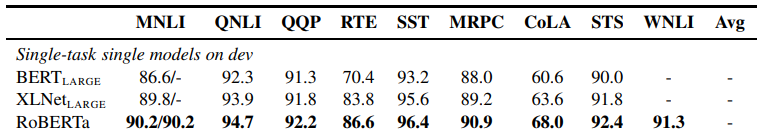
\includegraphics[width=0.6\textwidth]{../images/roberta-tasks.png}
    \caption{TODO}
    \label{fig:bert-vs-roberta-paper}
\end{figure}

The results of the paper show RoBERTa beats BERT in all given Natural Language Processing tasks. In this project similar tests
were carried out on the specific topic classification task. The results of the classification were
compared to see which model performed better.
\begin{figure}[hbtp]
    \centering
    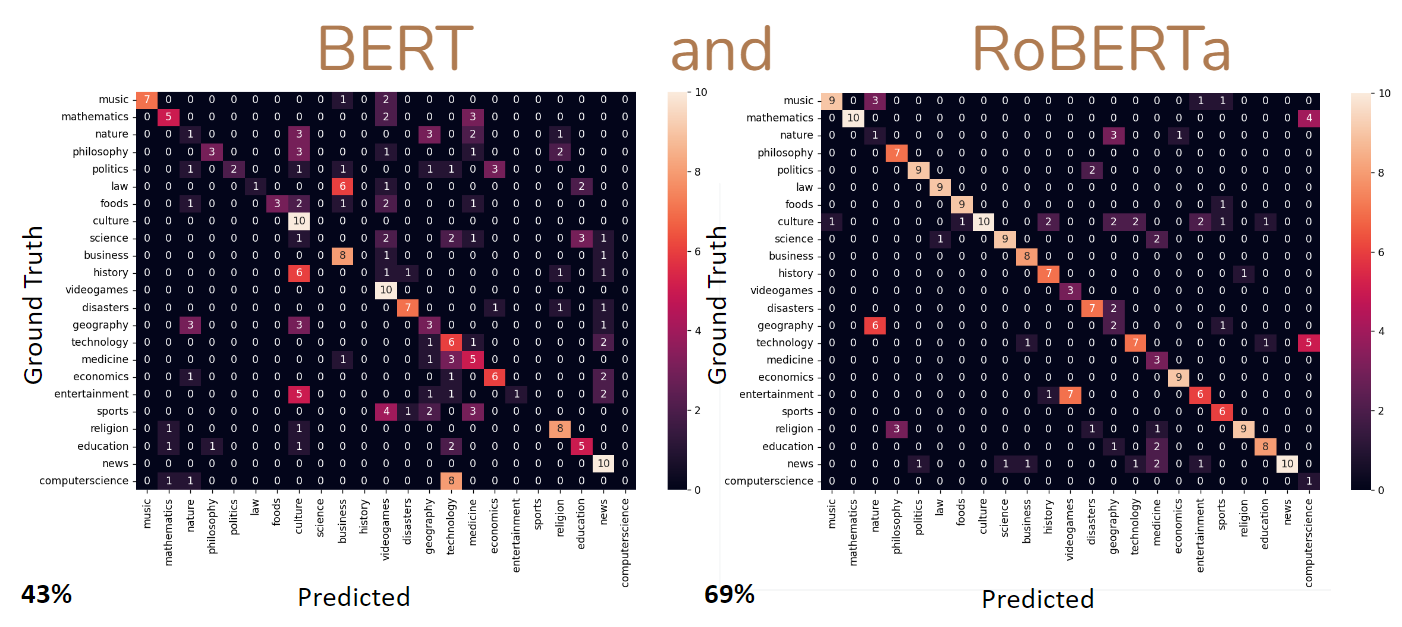
\includegraphics[width=0.6\textwidth]{../images/bert-vs-roberta.png}
    \caption{BERT vs RoBERTa}
    \label{fig:bert-vs-roberta}
\end{figure}

Figure \ref{fig:bert-vs-roberta} shows the confusion matrices of BERT and RoBERTa respectively for the test set - the test set was a
random 10\% sample of the training data. The columns of the confusion matrix represent the predicted labels and the rows represent the
ground truth labels. It is obvious from the confusion matrices that BERT did not perform as well as RoBERTa; there are a lot of
misclassifications. A misclassification can be identified as a cell in the confusion matrix that is not on the diagonal. Comparing this
to the confusion matrix of RoBERTa, it is clear that RoBERTa performed much better. In fact, RoBERTa is $60\%$ more accurate than BERT
($43\%$ compared to $69\%$).
\section{Principal Component Analysis (PCA) of data}
One thing to note in the RoBERTa confusion matrix in Figure \ref{fig:bert-vs-roberta} is that the model has high concentration
of misclassifications; the model makes the same misclassification often. After noticing this trend, it was believed that the topics
that were commonly misclassified were similar to each other - could be grouped together.\\
Principal Component Analysis (PCA) was used to reduce the dimensionality of the data and to allow for visualisation of the data. PCA
was performed on the output features of RoBERTa.
\begin{figure}
    \centering
    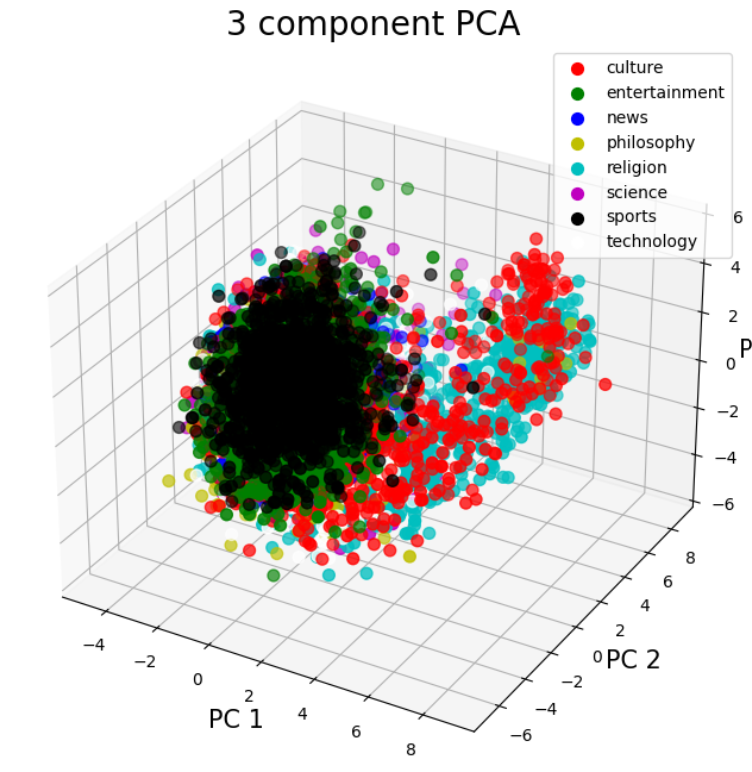
\includegraphics[width=0.6\textwidth]{../images/pca.png}
    \caption{PCA of data}
    \label{fig:pca}
\end{figure}

Figure \ref{fig:pca} shows the PCA of the data. The data was reduced to 3 dimensions using PCA. The data was then plotted on a 3D
graph. The colours of the points represent the topics (of which some are identified in the legend). The graph is not easy to interpret;
the only visible trend is that `Religion' and `Culture' seem to be very dissimilar to the other topics.\\
To help interpret the data, the analysis was performed on 2 topics at a time. This time the data was reduced to 2 dimensions using
PCA. The data was then plotted on a 2D graph.
\subsection{Findings from PCA}
In this section, the notable findings from the PCA are discussed.
\subsubsection{Mathematics vs Music}
This comparison was made to act as a baseline for the rest of the comparisons. The hypothesis was that these topics would be
dissimilar to each other.
\begin{figure}
    \centering
    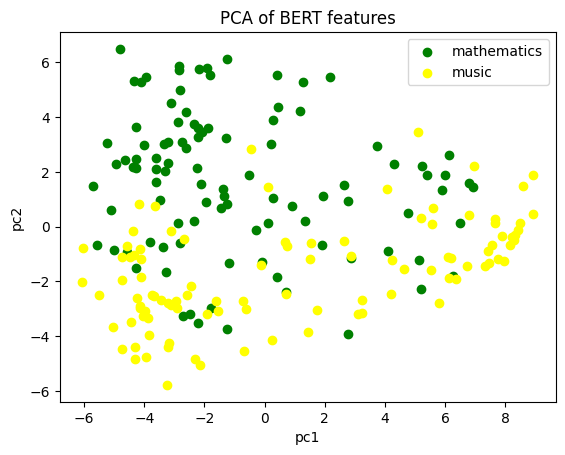
\includegraphics[width=0.6\textwidth]{../images/math-vs-music.png}
    \caption{Mathematics vs Music}
    \label{fig:math-vs-music}
\end{figure}

Figure \ref{fig:math-vs-music} shows the PCA of the data for the `Mathematics' and `Music' topics. There is a clear separation between
the two topics. Although the data is not linearly separable, there is a strong trend that the data points of the `Mathematics' topic
are on the bottom of the graph and the data points of the `Music' topic are on the top of the graph. Using a perceptron classifier
on the 2 principal components, led to an accuracy of $73\%$. This is a strong indicator that the 2 topics are dissimilar to each other.
\subsubsection{Geography vs Nature}
Looking back at the confusion matrix of RoBERTa in Figure \ref{fig:bert-vs-roberta}, the model predicts `Geography' instead of
`Nature' 6 times out of 10. This is a very high concentration of misclassifications. The hypothesis was that the topics are very similar.
\begin{figure}
    \centering
    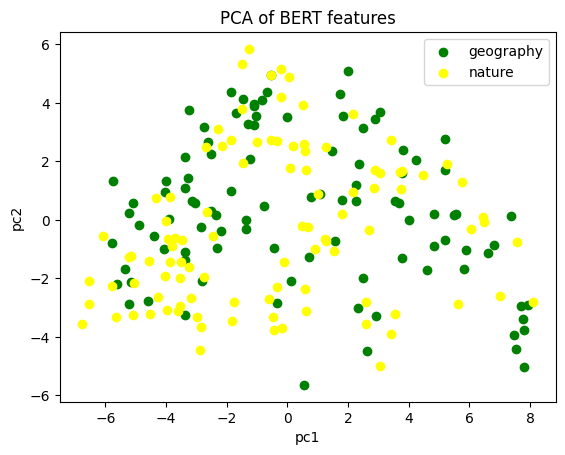
\includegraphics[width=0.6\textwidth]{../images/geography-vs-nature.png}
    \caption{Geography vs Nature}
    \label{fig:geography-vs-nature}
\end{figure}

The figure shows the PCA of the data for the `Geography' and `Nature' topics. In comparison to Figure \ref{fig:math-vs-music}, there is
no clear separation between the two topics. In fact, visually, the two topics seem to be almost identical. Using a perceptron classifier
on the 2 principal components, led to an accuracy of $52\%$. This is a strong indicator that the 2 topics are similar; the fact the classifier
is only a minor improvement on random guessing shows that the 2 topics are similar.\\
From this finding it was concluded that the model was not able to distinguish between the two topics. This led to the merging of the
`Geography' and `Nature' topics into a single topic. It was decided this topic would be called `Geography'.
\subsubsection{Technology vs Computer Science}
Similarly to the previous comparison, the confusion matrix in Figure \ref{fig:bert-vs-roberta} shows that the model predicts `Technology'
instead of `Computer Science' 5 times out of 10. The hypothesis was that the topics are very similar. However, the results from the 
perceptron classifier on the 2 principal components showed a very high accuracy of (TODO). This is not the result expected and caused
confusion as to why the model was unable to distinguish between the two topics.\\
To further investigate this, the data was manually inspected to attempt to reach a new hypothesis. This led to the discovery of the 
unbalanced nature of the data. The `Technology' topic had 10 times more data points than the `Computer Science' topic. This answers why
the perceptron classifier performed so well but the model was unable to distinguish between the two topics.\\
The inbalance of the data was a surprise as the script used to scrape the data was designed to scrape an equal number of data points.
It was found that the search query for the `Computer Science' topic yielded no results on wikipedia leading to a small number of data
points.\\
It was decided to remove the computer science topic from the dataset due to the limited dataset.
\subsubsection{News}
TODO
\section{Context}
\subsection{Media - Images and Videos}
After implementing OCR and Wav2Vec, the model was tested on a set of 60 hand picked posts (3 for each topic). The updated context aware
model was compared to the original model.
\begin{figure}
    \centering
    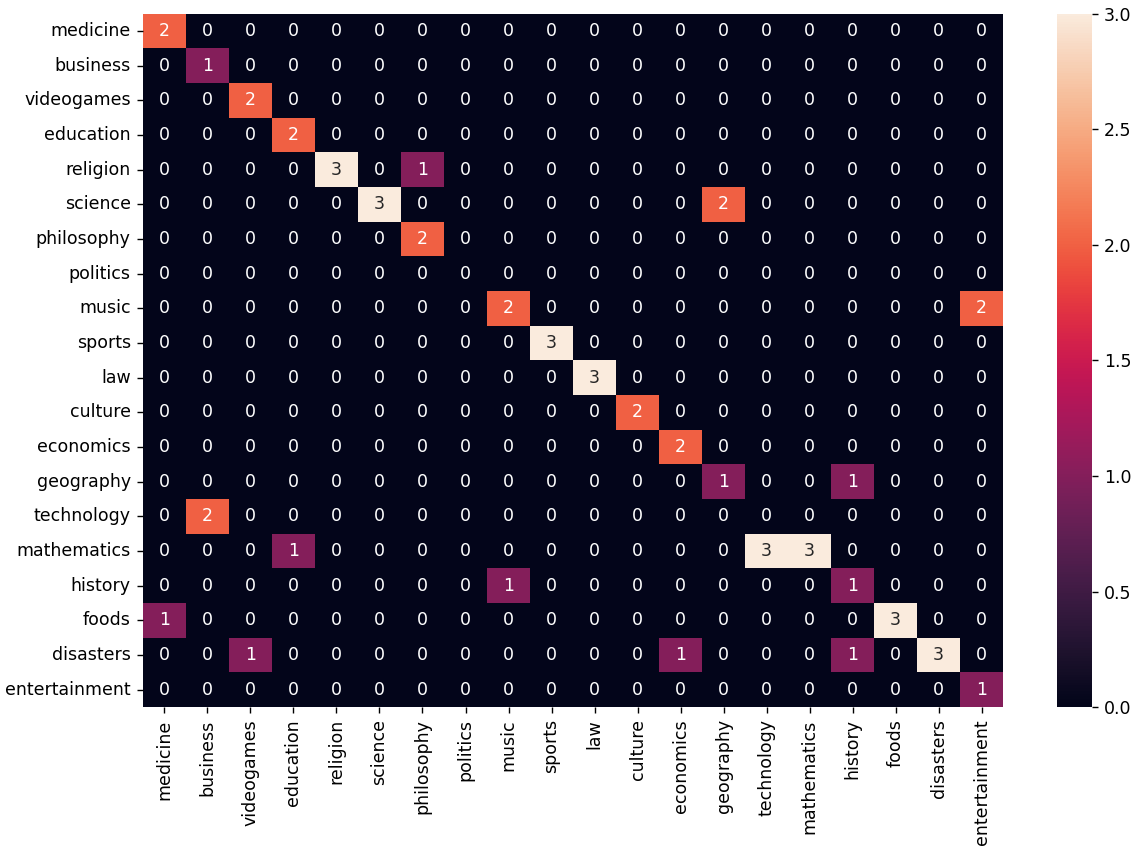
\includegraphics[width=0.6\textwidth]{../images/confusion/Complete-no-media-confusion.png}
    \caption{Confusion Matrix without Media Context}
    \label{fig:confusion}
\end{figure}
\begin{figure}
    \centering
    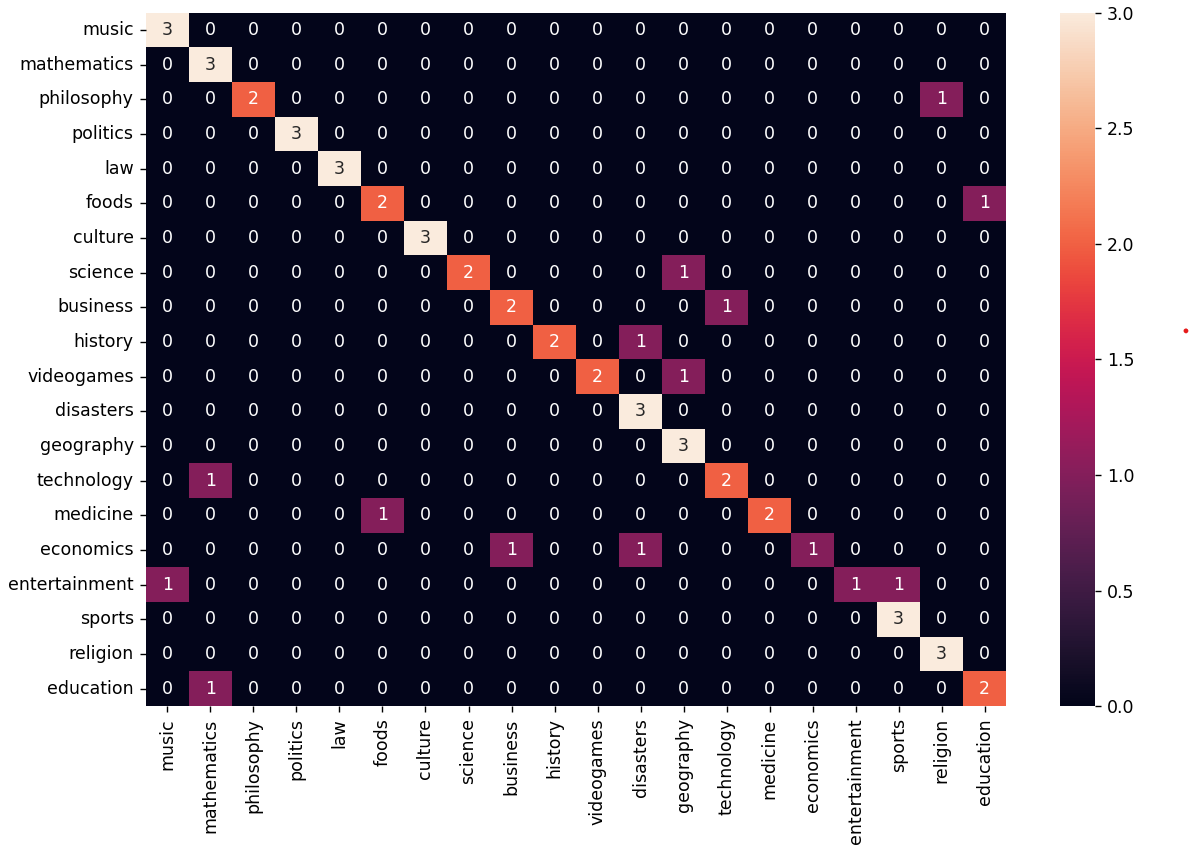
\includegraphics[width=0.6\textwidth]{../images/confusion/Complete-Model-test.png}
    \caption{Confusion Matrix with Media Context}
    \label{fig:media}
\end{figure}

Figure \ref{fig:confusion} shows the confusion matrix of the original model. Figure \ref{fig:media} shows the confusion matrix of the
updated context aware model. The addition of the media context improved the accuracy of the model by $10\%$. This is a notable increase
in accuracy. However, due to the nature of gathering this test data, it must be noted some form of bias is present. The test data was
hand picked, so some unconscious bias may have been introduced to provide posts that would be hard to classify without the media,
but easy to classify with the media. Although, this could be the case this test does show that the context from media can still be useful
in classifying posts.\\
\subsection{Retweets and Threads}
Separately to implementing OCR and Wave2Vec, another model was created that added the context of retweets and threads. This model was
made separately to allow us to see the performance impact of the retweet and thread context. If we had tested them together, we would
have seen an improvement but would not have been able to identify the impact of each feature.\\
The model was tested on a set of 60 hand picked posts, that were different to the posts used in the previous test. The reason behind
this is simply the API used to access the tweets was unable to access retweets and threads from posts older than 7 days - The posts
used in the previous test were all older than 7 days when this test was performed.
\begin{figure}
    \centering
    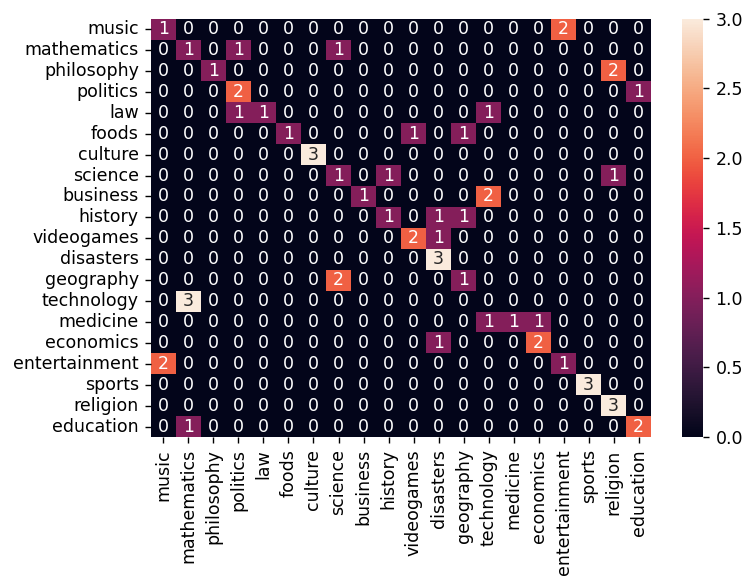
\includegraphics[width=0.6\textwidth]{../images/confusion/RoBERTa-nothread-20.png}
    \caption{Confusion Matrix without Thread/Retweet Context}
    \label{fig:confusion2}
\end{figure}
\begin{figure}
    \centering
    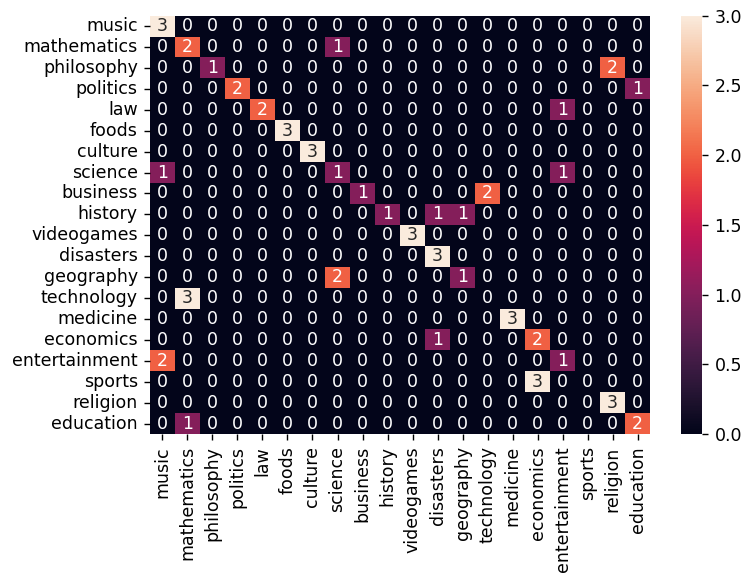
\includegraphics[width=0.6\textwidth]{../images/confusion/RoBERTa-thread-20.png}
    \caption{Confusion Matrix with Thread/Retweet Context}
    \label{fig:retweet}
\end{figure}

Figure \ref{fig:confusion2} shows the confusion matrix of the original model. Figure \ref{fig:retweet} shows the confusion matrix of the
thread/retweet context aware model. Similarly to the previous test, the addition of the thread/retweet context improved the accuracy of
the model by $10\%$. Again, this is a notable increase in accuracy although the same bias as the previous test is present.

\subsection{Context Aware Conclusion}
The context aware models both improved the accuracy of the model by $10\%$. This shows how this extra context can be useful in
classifying posts. However, there are cases where the extra context is not useful. For example, some videos are paired with songs for
their audio. This audio is not related to the topic of the post. Which could cause the model to misclassify the post. In its current state
the model is not able to identify whether the audio is related to the topic of the post or not.\\
This project shows that the context of the post can be useful in classifying posts. However, due to the naive approach taken
in this project, the context is not always useful. In \Cref{ch:conclusions} we will discuss how this context can be used in a more
sophisticated way to improve the accuracy of the model.